% !TeX root = ../../main.tex
\section{设计计算与校核}

\subsection{脉冲器计算与校核}

脉冲器设计要求如下表所示。

\begin{table}[htbp]
    \centering
    \caption{脉冲器设计要求}
    \label{tab:pulsar_design_req}
    \renewcommand{\arraystretch}{1.5} % 增加行高，使表格更美观
    \begin{tabularx}{1.0\textwidth}{ccXccc}
        \toprule % 顶线
        \begin{tabular}[c]{@{}c@{}}外径\\ (mm)\end{tabular} & 
        \begin{tabular}[c]{@{}c@{}}水眼直径\\ (mm)\end{tabular} & 
        接头螺纹扣型 & 
        \begin{tabular}[c]{@{}c@{}}许用拉力\\ (kN)\end{tabular} & 
        \begin{tabular}[c]{@{}c@{}}许用扭矩\\ ($\text{kN}\cdot\text{m}$)\end{tabular} & 
        \begin{tabular}[c]{@{}c@{}}总长\\ (mm)\end{tabular} \\
        \midrule % 栏目线
        105 & 25 & NC31 & 400 & 8 & 1250 \\
        \bottomrule % 底线
    \end{tabularx}
\end{table}


该产品为井下清洁工具，工作条件十分恶劣，其结构属于中间空的细长杆件且筒体较薄。依据API标准对钻具的材料要求，选用具有较高强度的4145H合金结构钢并经调质处理，作为产品的主体结构材料，钢材成分应符合ASTM A304-05e2标准的规定。
为适应工作条件下的应力状态，热处理后的力学性能应达到以下要求。

\begin{table}[htbp]
    \centering
    \caption{产品要求}
    \label{tab:product_requirements}
    \renewcommand{\arraystretch}{1.5} % 增加行高，使表格更美观
    \begin{tabularx}{1.0\textwidth}{cXcc}
        \toprule % 顶线
        硬度 & 最小屈服强度 & 伸长率 & 夏比冲击功 \\
        \midrule % 栏目线
        285-321(HB) & $\sigma_S \ge 785\text{MPa}$ & $13\%$ & $Akv \ge 54\text{J}$ \\
        \bottomrule % 底线
    \end{tabularx}
\end{table}


1） 危险截面（螺纹应力分散槽处）抗拉抗扭计算

（1）许用拉力计算

\begin{equation}
    F_{\max} = \frac{[\pi \cdot (D^2 - d^2)] \cdot \sigma_s}{4 \cdot n} \times 10^{-3}
\end{equation}
式中，$F_{\max}$为工具最大拉力，$\mathrm{kN}$；

$D$为危险截面外径，$\mathrm{mm}$；

$d$为危险截面内径，$\mathrm{mm}$；

$\sigma_s$为材料最小屈服强度，取825 MPa（4145H）；

$n$为安全系数，取$n = 1.5$。

代入数据计算如下：
\begin{equation}
\begin{aligned}
    F_{\max} &= \frac{\pi \cdot (D^2 - d^2) \cdot \sigma_s}{4 \cdot n} \times 10^{-3} \\
             &= \frac{3.14 \times (50^2 - 30^2) \times 825}{4 \times 1.5} \times 10^{-3} \\
             &= 690.8 \, \text{kN} > 400 \, \text{kN}
\end{aligned}
\end{equation}
满足设计要求。

(2) 许用扭矩计算

\begin{equation}
    T_{\max} = \frac{\sigma_s \cdot \pi \cdot (D^4 - d^4)}{16 \cdot D \cdot n} \times 10^{-6}
\end{equation}
式中，$T_{\max}$为最大扭矩，$\mathrm{kN\cdot m}$；

$\sigma_s$为材料屈服应力，$\mathrm{MPa}$；

$D$为危险截面外径，$\mathrm{mm}$；

$d$为危险截面内径，$\mathrm{mm}$；

$n$为安全系数，根据《机械设计手册》机械零部件强度计算中安全系数的取值规定\cite{ref26}，取$n = 1.5$。

代入数据计算得：
\begin{equation}
\begin{aligned}
    T_{\max} &= \frac{\sigma_s \cdot \pi \cdot (D^4 - d^4)}{16 \cdot D \cdot n} \times 10^{-6} \\
             &= \frac{825 \times 3.14 \times (50^4 - 30^4)}{16 \times 50 \times 1.5} \times 10^{-6} \\
             &= 11.74 \, \text{kN} \cdot \text{m} > 8 \, \text{kN} \cdot \text{m} 
\end{aligned}
\end{equation}
满足设计要求。

2）主要受力件仿真校核

脉冲器的主要受力件为脉冲器心轴，危险截面出现在出水口，脉冲器芯轴的最大拉应力为630MPa，小于设计要求，最大切应力为994MPa，但范围极小，属于应力集中导致的局部小尺度高应力，不会引发整体塑性变形；强度满足设计要求。


\begin{figure}[htbp]
	\centering
	\subfloat[脉冲器心轴]{%
	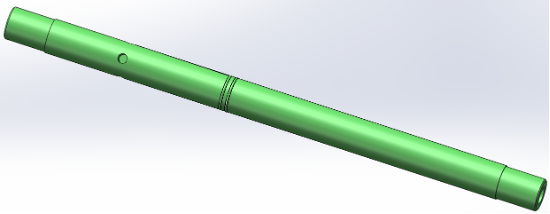
\includegraphics[width=0.7\textwidth]{figure/chapter3/inner-pipe-3-in-1.png}
	}
	\hfill
	\subfloat[抗拉强度分析]{%
	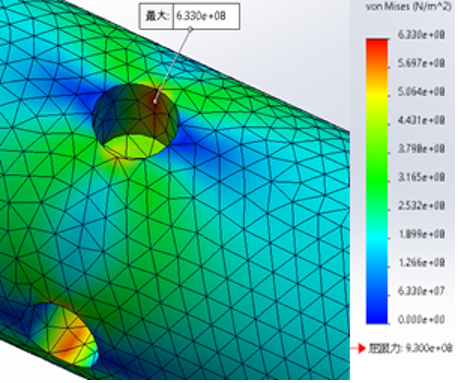
\includegraphics[width=0.4\textwidth]{figure/chapter3/inner-pipe-3-in-1-tensile-stress.png}
	}
	\vspace{1em}
	\subfloat[抗扭强度分析]{%
	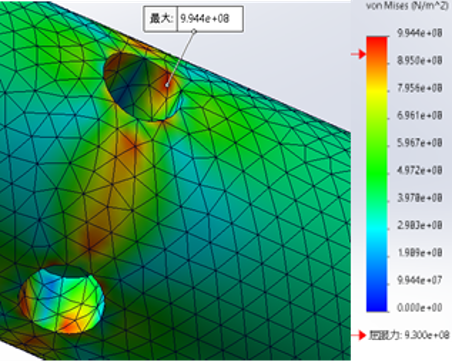
\includegraphics[width=0.45\textwidth]{figure/chapter3/inner-pipe-3-in-1-torsional-stress.png}
	}
	\caption{脉冲发生器薄弱零件强度有限元分析}
	\label{fig:FEA_inner_pipe_3_in_1}
\end{figure}
